\documentclass[12pt,a4paper]{ctexart}

% ========== 页面设置 ==========
\usepackage[a4paper,margin=2.5cm]{geometry}
\usepackage{setspace}
\usepackage{enumitem}
\usepackage{graphicx}  % 插入图片的宏包
\usepackage{titlesec}
\usepackage{amsmath,amssymb}
\usepackage{fontspec}
\usepackage{fancyhdr}          % 控制页眉页脚
\usepackage[hidelinks]{hyperref}
\usepackage[backend=biber,style=ieee]{biblatex}

% bib
\addbibresource{references.bib}

% ========== 字体设置 ==========
\setmainfont{Times New Roman} % 英文主字体
\setCJKmainfont{SimSun}       % 中文主字体：宋体

% ========== 段落与格式 ==========
\setlength{\parindent}{2em}
\setlength{\parskip}{0.8em}
\linespread{1.3}  % 行距

% ========== 标题格式 ==========
\titleformat{\section}
  {\bfseries\large}
  {\thesection、}
  {0.5em}
  {}

\titleformat{\subsection}
  {\normalsize}
  {\thesubsection\quad}
  {0em}
  {}

% 页眉，页脚
\pagestyle{fancy}                   % 启用 fancy 样式
\fancyhf{}                          % 清空原有页眉页脚
\fancyfoot[C]{\thepage}             % 页脚中间显示页码
\renewcommand{\headrulewidth}{0pt}  % 去掉页眉横线
\renewcommand{\footrulewidth}{0pt}  % 去掉页脚横线（可选）

% ========== 正文 ==========
\begin{document}

\begin{center}
    \LARGE \textbf{高等数字集成电路作业-2025-1}
\end{center}

\section{基础概念问题}

\subsection{请简要描述集成电路设计过程中，抽象分层的常规做法？抽象分层对集成电路设计所带来的意义何在？结合自己对设计的理解阐述抽象分层的方法和意义？}

集成电路设计中，常规分层方法包括，系统层、模块层级、门电路层级、电路层级、器件级。抽象分层的意义是将复杂的系统设计简单化，提高设计开发效率。

集成电路设计过程的抽象分层，抽象分层是自顶向下，层层递进的。对设计而言，用于分配的设计任务粒度是模块层级，所以在系统层（top）对集成电路的逻辑功能进行模块化分层是最关键的一步，需要考虑如何划分模块能尽可能的解耦逻辑功能，还要保证各个模块的功能足够简洁，同时分层策略最终要服务于系统层功能的实现。

抽象分层最大的意义就是提高开发效率，此外也有利于提高系统的可拓展性、稳健性以及可维护性等。在系统层进行大型设计的集成仿真测试、综合是十分耗时的，同时也难以定位问题。抽象分层后，按照模块进行开发，各个模块有更小粒度的设计指标，可以独立进行设计、验证。保证模块层级妥善后再进行系统层的验证，大幅提高设计效率，降低问题定位难度。


\subsection{请简要描述为何典型的超大规模集成电路，通常是采用 CMOS 工艺为基础进行的设计，而不是采用基于其他工艺为基础进行 VLSI 设计？CMOS 电路的优势是什么？}

典型超大规模集成电路采用CMOS工艺的主要原因是其低功耗与高噪声容限的优势。在CMOS之前采用的工艺有TTL、单MOS，TTL和单MOS都有较高的静态功耗，而CMOS电路的互补结构使其静态功耗基本为0。此外，互补结构能够保证输出电压范围为完整的VDD,逻辑阈值可以接近VDD中点，可以容忍较大的干扰，意味着可以工作在更低的电压。以上亮点最终都有利于降低CMOS电路的功耗，有利于提高CMOD电路的集成度。

\subsection{请通过查阅文献，介绍MOS器件、NMOS器件、PMOS器件、CMOS器件、CMOS集成电路的发明历史、发明人、对行业发展带来的促进意义，CMOS技术发展演进的若干行业标志性事件，对CMOS集成电路发明直至规模应用的几位关键工程专家的发明或发现的关键事件做介绍，详细阅读CMOS的几篇关键文献并对CMOS器件发明的科研学术及工程价值做总结阐述。}

MOS器件最早由Dawon Kahng与Martin M.Atalla于1959年在贝尔实验室成功制造\cite{mos,mos_patent}，同时实现了n型沟道和p型沟道器件，实现了NMOS和PMOS器件的原型。他们利用高质量的二氧化硅薄膜作为栅介质，首次解决了硅表面态导致的漏电与失效问题，使得MOS结构成为可量产的基础器件。MOS器件的发明标志着半导体器件从双极型晶体管时代迈入场效应管时代，为后续的大规模集成电路奠定了物理与工艺基础。CMOS器件工艺概念最早由仙童半导体的Frank Wanlass 与 Chih-Tang Sah在1963年的ISSCC会议上阐述\cite{cmos}，1967年Wanlass关于CMOS的专利得到授权\cite{cmos_patent}。PMOS和NMOS的互补特性使其具有低功耗与高集成特性，彻底改变了集成电路的发展轨迹。

在CMOS集成电路工艺概念提出之后，CMOS集成电路技术很快被产业界注意并实现商业化。1966年，RCA公司将 CMOS 应用于通用逻辑器件，并推出了著名的 CD4000系列 CMOS 逻辑器件，从而把 CMOS 技术推向市场并被广泛采用。1965年，英特尔公司联合创始人 Gordon E. Moore 在《Electronics》杂志上发表文章\cite{moore}，提出了著名的摩尔定律，指出集成电路上可容纳的晶体管数量大约每隔 18 至 24 个月会增加一倍，而成本保持不变或下降。该规律揭示了半导体技术持续微缩和性能提升的指数级发展趋势，成为半导体产业的重要指导原则，推动了集成电路技术的快速进步，加速了现代信息社会的形成。然而，随着 CMOS 工艺节点不断缩小传统平面 MOSFET 出现严重的短沟道效应和漏电流问题，鳍式场效应晶体管（FinFET）的MOSFET工艺被提出，通过3D结构继续延伸上限，延续摩尔定律。FinFET最早由Yutaka Hayashi于1980年在日本筑波的电工实验室发明并提交专利，1984年发表文章\cite{finfet}进行阐述。

CMOS器件的发明，是半导体科学与工程史上的里程碑事件，其科研与工程价值体现在从物理原理、设计理念到产业体系的全面革新。在科研层面，CMOS 的提出将电路功耗问题与器件物理本质紧密联系，开创了低功耗电路的全新范式。其互补对称结构使得电路在静态条件下几乎不消耗功率，仅在开关瞬间产生动态能耗，这一特性奠定了大规模集成电路的基础。从工程角度来看，CMOS 技术的核心价值在于它构建了一个可持续微缩、兼具低功耗与高密度特性的器件平台。凭借工艺兼容性和对称性，CMOS 成为集成电路从中小规模向超大规模演进的关键支撑技术。为延续 CMOS 技术的发展轨迹，CMOS技术也在不断改进，如FinFET工艺技术标志着 CMOS 技术在三维结构维度上的一次重大演化。

CMOS工艺标准化和兼容性促进了全球半导体产业链的形成与成熟，催生了集成电路设计、EDA 工具、晶圆制造与封测等完整生态体系，推动了现代信息技术产业的快速发展，几乎所有现代电子设备的核心逻辑都基于 CMOS 技术。

\subsection{请分析针对CMOS反相器电路设计优化，在输出驱动一定的前提下，通过哪些技术手段可提高CMOS反相器的驱动能力？ }

最简单的反相器电路由最基本的CMOS电路单元组成，即一个NMOS与一个PMOS。然而，单个CMOS单元的驱动能力是有限的，在集成电路中可以通过逐级堆叠的反相器链提高CMOS的反相器驱动能力，以CMOS反相器链的版图\ref{fig:invx8}为例，输入信号A经过三个反相器CMOS单元，这三个单元分别由1、2、4个NMOS和PMOS单元并行组成，其最终输出驱动能力得到提升。

\begin{figure}[htbp]
    \centering
    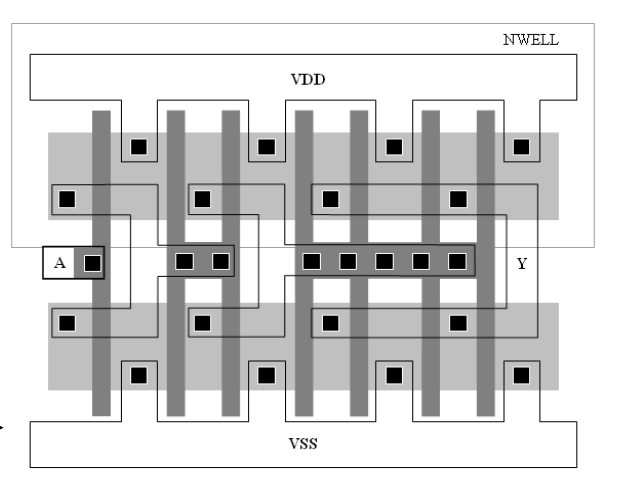
\includegraphics[width=0.6\textwidth]{figure/invx8.png}
    \caption{反相器链设计版图}
    \label{fig:invx8}
\end{figure}

\subsection{请简要描述在CMOS电路设计过程中，如何避免或降低寄生电感引起的同步开关噪声（SSN）所导致的电路性能不稳定？}

SSN的本质是由于大量CMOS输出同时翻转，导致瞬时电源电流变化过大，电源与地间的寄生电感产生电压扰动，使得实际VDD降低、地电位上升，造成电源噪声。因此，通过增加VDD与GND引脚个数，降低单个VDD引脚上的电流，或使用芯片时在IC引脚增加去耦电容。

\subsection{请说明为何在绝大部分VLSI电路设计过程中，都使用的同步电路而非异步电路，同步电路与异步电路各自优劣势。}

同步电路设计简单、电路可靠以及便于模块化设计，并且，同步电路的电路模型简单，方便使用EDA工具进行仿真、分析等。然而，同步电路中所有的电路工作在固定的时钟频率，时序松弛的模块被迫工作在高频下，额外导致了大量的功耗，需要高频响应的电路也被迫工作在固定频率，响应时间会受到限制。而异步电路允许不同模块使用不同的时钟域、能够让各个电路定制化设计，降低系统功耗，但其时序分析较为复杂，系统中异步电路的集成也需要额外的电路面积实现。

\subsection{请简要描述ASIC/FPGA前端设计流程？简要描述Top-Down设计流程的意义及挑战？}

\printbibliography

\end{document}

